\documentclass[../main.tex]{subfiles}
% !TeX root = ../main.tex
\begin{document}
	\section{Cash and Internal Controls}
	
	\subsection{Internal Control System}
	
	Managers use an internal control system to monitor and control business 
	activities.  An \textbf{internal control system} consists of the policies 
	and procedures managers use to: 
	\begin{itemize}[noitemsep]
		\item Protect assets.
		\item Ensure reliable accounting.
		\item Promote efficient operations.
		\item Urge adherence to company policies.
	\end{itemize}
	
	Internal Controls provides protection from fraud, waste, and inefficiency.
	Companies can do business in a trustworthy manner that ensures public 
	confidence - an extremely important element in maintaining the stability of 
	financial markets around the world.
	
	\subsubsection{Principles of Internal Control}
	
	Internal control policies and procedures vary from company to company 
	according to such factors as the nature of the business and its size. 
	Certain fundamental internal control principles apply to all companies. The 
	principles of internal control are to:
	\begin{itemize}[noitemsep]
		\item \textbf{Establish responsibilities.} Proper internal control 
		means that responsibility for a task is clearly established and 
		assigned to one person.
		\item \textbf{Maintain adequate records.} Good record-keeping is part 
		of an internal control system. It helps protect assets and ensures that 
		employees use prescribed procedures.
		\item \textbf{Insure assets and bond key employees.} Good internal 
		control means 
		that assets are adequately insured against casualty and that employees 
		handling  large amounts of cash and easily transferable assets are 
		bonded.
		\item \textbf{Separate record-keeping from custody of assets.} A person 
		who controls or has access to an asset must not keep that asset’s 
		accounting records.
		\item \textbf{Divide responsibility for related transactions.} Good 
		internal control divides responsibility for a transaction or a series 
		of related transactions between two or more individuals or departments.
		\item \textbf{Apply technological controls.} Cash registers, check 
		protectors, time clocks, and personal identification scanners are 
		examples of devices that can improve internal control.
		\item \textbf{Perform regular and independent reviews.} Changes in 
		personnel, technological advances, and normal business pressures for 
		performance necessitate reviews to ensure that proper procedures are 
		being followed on a consistent basis.
	\end{itemize}

	\subsubsection{Technology and Internal Control}
	
	The fundamental principles of internal control are relevant no matter what 
	the technological state of the accounting system, from purely manual to 
	fully automated systems. Technology impacts an internal control system in 
	several important ways. Perhaps the most obvious is that technology allows 
	us quicker access to databases and information. Used effectively, 
	technology greatly improves managers’ abilities to monitor and control 
	business activities:
	\begin{itemize}[noitemsep]
		\item \textbf{Reduced Processing Errors.} Technologically advanced 
		systems 
		reduce the 
		number of errors in processing information. Provided the software and 
		data entry are correct, the risk of mechanical and mathematical errors 
		is nearly eliminated.
		\item \textbf{
			More Extensive Testing of Records.} A company’s review and audit of 
			electronic records can include more extensive testing when 
			information is easily and rapidly accessed.
		\item \textbf{Limited Evidence of Processing.} Many data processing 
		steps are increasingly done by computer. Accordingly, fewer hard-copy 
		items of documentary evidence are available for review. Yet 
		technologically advanced systems can provide new evidence. They can, 
		for instance, record who made the entries, the date and time, the 
		source of the entry, and so on.
		\item \textbf{Crucial Separation of Duties.} Technological advances in 
		accounting 
		information systems often yield some job eliminations or 
		consolidations. While those who remain have the special skills 
		necessary to operate advanced programs and equipment, a company with a 
		reduced workforce risks losing its crucial separation of duties. The 
		company must establish ways to control and monitor employees to 
		minimize risk of error and fraud.
		\item \textbf{Increased E-Commerce.} Most companies have some 
		e-commerce 
		transactions. All such transactions involve at least three risks. 
		\begin{itemize}[noitemsep]
			\item \textbf{Credit card number theft} is a risk of using, 
			transmitting, 
			and storing such data online. This increases the cost of e-commerce.
			\item \textbf{Computer 
			viruses} are malicious programs that attach themselves to innocent 
			files 
			for purposes of infecting and harming other files and programs.
			\item \textbf{Impersonation online} can result in charges of sales 
			to bogus accounts, 
			purchases of inappropriate materials, and the unknowing giving up 
			of 
			confidential information to hackers. Companies use both firewalls 
			and 
			encryption to combat some of these risks—firewalls are points of 
			entry 
			to a system that require passwords to continue, and encryption is a 
			mathematical process to rearrange contents that cannot be read 
			without 
			the process code.
		\end{itemize}
	\end{itemize}
	
	\subsubsection{Limitations of Internal Control}
	
	Internal control policies and procedures are applied by people. This human 
	element creates several potential limitations that we can categorize as 
	either:
	\begin{itemize}[noitemsep]
		\item \textbf{Human Error} can occur from negligence, fatigue, 
		misjudgment, or confusion.
		\item \textbf{Human fraud} involves intent by people to defeat internal 
		controls, such as management override, for personal gain. 
		\textbf{Fraud} is an 
		intentional misrepresentation of facts, made for the purpose of 
		persuading another party to act in a way that causes injury or damage 
		to that party. Fraud is a huge problem and is getting bigger across the 
		globe. Fraud has exploded with the expansion of e-commerce via the 
		Internet. Human fraud is driven by the triple-threat of fraud:
		\begin{itemize}[noitemsep]
			\item \textbf{Opportunity} - refers to internal control 
			deficiencies in the workplace. 
			\item \textbf{Pressure} - refers to financial, family, society, and 
			other stresses to succeed.  
			\item \textbf{Rationalization} - refers to employees rationalizing 
			fraudulent behavior. 
		\end{itemize}
	\end{itemize}

	\paragraph{Fraud.} The two most common types of fraud that impact the 
	financial statements are misappropriation of assets and fraudulent 
	financial reporting. 
	\begin{itemize}[noitemsep]
		\item \textbf{Misappropriation of assets} is committed by employees of 
		an entity who steal money from the company and cover it up through 
		erroneous entries in the books \eg employee theft of inventory, bribery 
		or kickback schemes in the purchasing function, or employee 
		overstatement of expense reimbursement requests.
		\item \textbf{Fraudulent financial reporting} is committed by company 
		managers who make false and misleading entries in the books, making 
		financial results of the company appear to be better than they actually 
		are. The purpose of this type of fraud is to deceive investors and 
		creditors into investing or loaning money to the company that they 
		might not otherwise have invested or loaned.
	\end{itemize}
	
	The second major limitation on internal control is the \textbf{cost–benefit 
	principle}, which dictates that the costs of internal controls must not 
	exceed their benefits. Analysis of costs and benefits must consider all 
	factors, including the impact on morale. 
	
	Most companies, for instance, have 
	a legal right to read employees’ e-mails, yet companies seldom exercise 
	that right unless they are confronted with evidence of potential harm to 
	the company. The same holds for drug testing, phone tapping, and hidden 
	cameras. The bottom line is that managers must establish internal control 
	policies and procedures with a net benefit to the company.
	
	\subsection{Internal Control for Cash}
	
	Internal control for cash is important for two main reasons:
	\begin{itemize}[noitemsep]
		\item The volume of cash transactions is enormous, the risk of 
		cash-handling errors is significant.
		\item Cash is valuable, portable, and “owned” by the person who 
		possesses it, it poses a high risk of theft.
	\end{itemize}

	Cash is a necessary asset of every company. Most companies also own cash 
	equivalents (defined later), which are assets similar to cash. Cash and 
	cash equivalents are the most liquid of all assets and are easily hidden 
	and moved. An effective system of internal controls protects these assets 
	and it should meet three basic guidelines:
	\begin{itemize}[noitemsep]
		\item Handling cash is separate from record-keeping of cash.
		\item Cash receipts are promptly deposited in a bank.
		\item Cash disbursements are made by check.
	\end{itemize}
	
	\subsubsection{Cash, Cash Equivalents and Liquidity}
	
	Good accounting systems help in managing the amount of cash and controlling 
	who has access to it. Cash is the usual means of payment when paying for 
	assets, services, or liabilities. 
	
	\textbf{Liquidity} refers to a company’s ability 
	to pay for its near-term obligations. Cash and similar assets are called 
	\textbf{liquid assets} because they can be readily used to settle such 
	obligations. A company needs liquid assets to effectively operate. 
	
	\textbf{Cash} includes currency and coins along with the amounts on deposit 
	in bank 
	accounts, checking accounts (called demand deposits), and many savings 
	accounts (called time deposits). Cash also includes items that are 
	acceptable for deposit in these accounts such as customer checks, cashier 
	checks, certified checks, and money orders. 
	
	\textbf{Cash equivalents} are short-term, highly liquid investment assets 
	meeting 
	two criteria:
	\begin{itemize}[noitemsep]
		\item Readily convertible to known amounts of cash.
		\item Subject to an insignificant risk of changes in value.
	\end{itemize}
	Most companies combine cash equivalents with cash as a single item on the 
	statement of financial position. 
	
	\subsubsection{Reporting Cash}
	
	Cash, as reported on the balance sheet, includes cash deposited with banks, 
	petty cash on hand, and cash equivalents. Cash equivalents are short-term, 
	highly liquid investments purchased within three months of maturity. They 
	are considered equivalent to cash because they are both readily convertible 
	to known amounts of cash and so near to maturity that there is little risk 
	their value will change. 
	
	\begin{figure}[ht]
		\centering
		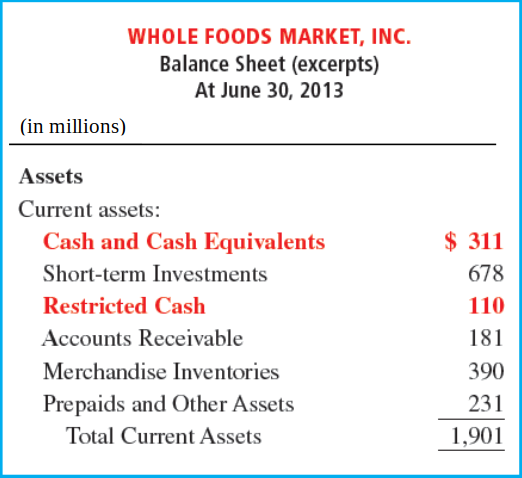
\includegraphics[width=0.7\columnwidth]{images/c5/reporting_cash.png}
		\caption{Reporting Cash on Balance Sheet}
	\end{figure}
	
	Companies are sometimes legally or contractually required to set aside cash 
	for a specific purpose and are not allowed to use it for day-to-day 
	operations. This \textbf{Restricted Cash} must be reported separately on 
	the balance sheet. Restricted cash is classified as a current asset because 
	it is expected to be used up within a year. Restricted cash that is not 
	expected to be used up within a year would be classified as a noncurrent 
	asset.
	
	\begin{figure}[ht]
		\centering
		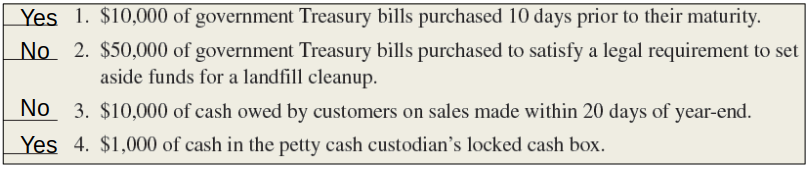
\includegraphics[width=1\columnwidth]{images/c5/reporting_cash_eg.png}
		\caption{Indicate Cash nd Cash Equivalents Example}
	\end{figure}
	
	\subsection{Cash Management}
	
	The goals of cash management are twofold:
	\begin{itemize}[noitemsep]
		\item Plan cash receipts to meet cash payments when due.
		\item Keep a minimum level fo cash necessary to operate. 
	\end{itemize}

	Effective cash management involves the following principles:
	\begin{itemize}[noitemsep]
		\item Encourage collection of receivables
		\item Delay payment of liabilities
		\item Keep only necessary level of assets
		\item Plan expenditures
		\item Invest excess cash
	\end{itemize}
	
	\subsection{Cash Receipts}
	
	The primary internal cash control goal for cash receipts is to ensure that 
	business receives the appropriate amount of cash and safely deposits it in 
	the bank. Businesses can receive Cash in two ways:
	\begin{itemize}[noitemsep]
		\item Receive cash in person at time of sale
		\item Receive cash through electronic transfer
	\end{itemize}
	
	\subsubsection{Over-the-Counter Cash Receipts}
	
	For purposes of internal control, over-the-counter cash receipts from sales 
	should be recorded on a cash register at the time of each sale. To help 
	ensure that correct amounts are entered, each register should be located so 
	customers can read the amounts entered. Clerks also should be required to 
	enter each sale before wrapping merchandise and to give the customer a 
	receipt for each sale. The design of each cash register should provide a 
	permanent, locked-in record of each transaction. In many systems, the 
	register is directly linked with computing and accounting services. Less 
	advanced registers simply print a record of each transaction on a paper 
	tape or electronic file locked inside the register. 
	
	\begin{figure}[ht]
		\centering
		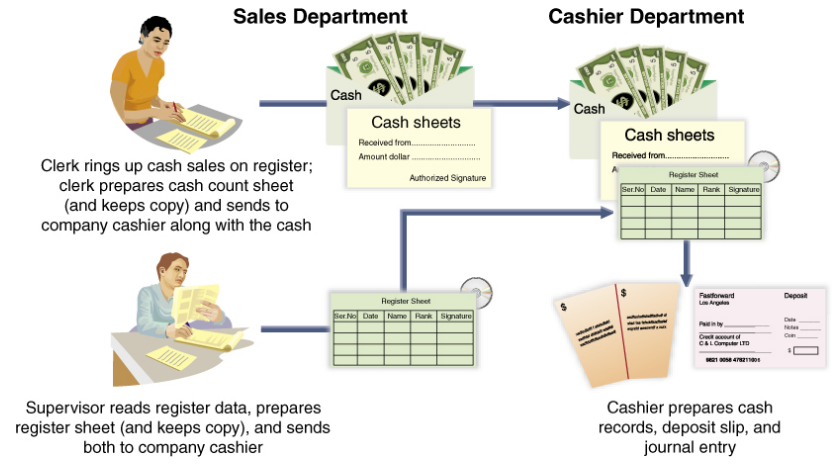
\includegraphics[width=1\columnwidth]{images/c5/otc_cash_receipts.png}
		\caption{Over-the-Counter Cash Receipts}
	\end{figure}
	
	Proper internal control prescribes that custody over cash should be 
	separate from its record-keeping. For over-the-counter cash receipts, this 
	separation begins with the cash sale. The clerk who has access to cash in 
	the register should not have access to its locked-in record. At the end of 
	the clerk’s work period, the clerk should count the cash in the register, 
	record the amount, and turn over the cash and a record of its amount to the 
	company cashier. The cashier, like the clerk, has access to the cash but 
	should not have access to accounting records (or the register tape or 
	file). A third employee, often a supervisor, compares the record of total 
	register transactions (or the register tape or file) with the cash receipts 
	reported by the cashier. This record is the basis for a journal entry 
	recording over-the-counter cash receipts. The third employee has access to 
	the records for cash but not to the actual cash. The clerk and the cashier 
	have access to cash but not to the accounting records. As this diagram 
	illustrates, none of them can make a mistake or divert cash without the 
	difference being revealed. 
	
	\subsubsection{Cash Over and Short}
	
	Sometimes errors in making change are discovered from differences between 
	the cash in a cash register and the record of the amount of cash receipts. 
	Although a clerk is careful, one or more customers can be given too much or 
	too little change. This means that at the end of a work period, the cash in 
	a cash register might not equal the record of cash receipts. This 
	difference is reported in the \textbf{Cash Over and Short} account, also 
	called \textbf{Cash Short and Over}, which is an income statement account 
	recording the income effects of cash overages and cash shortages.
	
	\begin{figure}[ht]
		\centering
		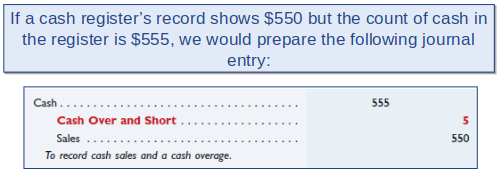
\includegraphics[width=1\columnwidth]{images/c5/cash_over_and_short.png}
	\end{figure}
	
	\subsubsection{Cash Receipts by Mail}
	
	Control of cash receipts that arrive through the mail starts with the 
	person who opens the mail. Preferably, two people are assigned the task of, 
	and are present for, opening the mail. In this case, theft of cash receipts 
	by mail requires collusion between these two employees. Specifically, the 
	person(s) opening the mail enters a list (in triplicate) of money received. 
	This list should contain a record of each sender’s name, the amount, and an 
	explanation of why the money is sent. The first copy is sent with the money 
	to the cashier. A second copy is sent to the recordkeeper in the accounting 
	area. A third copy is kept by the clerk(s) who opened the mail. The cashier 
	deposits the money in a bank, and the recordkeeper records the amounts 
	received in the accounting records. 
	
	\begin{figure}[ht]
		\centering
		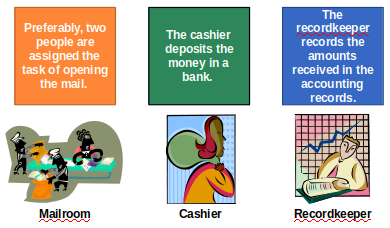
\includegraphics[width=0.8\columnwidth]{images/c5/mail_cash_receipts.png}
		\caption{Cash Receipts by Mail}
	\end{figure}
	
	When the bank balance is reconciled by another person (explained later), 
	errors or acts of fraud by the mail clerks, the cashier, or the 
	recordkeeper are revealed. They are revealed because the bank’s record of 
	cash deposited must agree with the records from each of the three. 
	Moreover, if the mail clerks do not report all receipts correctly, 
	customers will question their account balances. If the cashier does not 
	deposit all receipts, the bank balance does not agree with the 
	recordkeeper’s cash balance. The recordkeeper and the person who reconciles 
	the bank balance do not have access to cash and therefore have no 
	opportunity to divert cash to themselves. This system makes errors and 
	fraud highly unlikely. The exception is \textbf{employee collusion}.
	
	\subsection{Control of Cash Disbursements}
	
	Control of cash disbursements is especially important because most large 
	thefts occur from payment of fictitious invoices. The keys to controlling 
	cash disbursements are:
	\begin{itemize}[noitemsep]
		\item Require all expenditures to be made by check. The only exception 
		is small payments made from \textbf{petty cash}.
		\item Limit access to checks except for those who have the authority to 
		sign checks. A small business owner often signs checks and knows from 
		personal contact that the items being paid for are actually received. 
		This arrangement is impossible in large businesses. Instead, internal 
		control procedures must be substituted for personal contact. Such 
		procedures are designed to assure the check signer that the obligations 
		recorded are properly incurred and should be paid.
	\end{itemize}
	
	Most cash payments involve writing a check or completing an electronic 
	funds transfer (EFT). In rare cases where a company pays fro purchases with 
	dollar bills and coins, it uses a \textbf{petty cash system}. 
	
	The primary goal of internal controls for all cash payments is to ensure 
	that the business pays only for properly authorized transactions. 
	
	\subsubsection{Petty Cash System of Control}
	
	A basic principle for controlling cash disbursements is that all payments 
	must be made by check. An exception to this rule is made for \textbf{petty 
	cash disbursements}, which are the small payments required for items such 
	as postage, courier fees, minor repairs, and low-cost supplies.
	
	To avoid the time and cost of writing checks for small amounts, a company 
	sets up a petty cash fund to make small payments. Note that petty cash 
	activities are part of an \textbf{imprest system}, which designates advance 
	money to establish the fund, to withdraw from the fund, and to reimburse 
	the fund.
	
	To avoid the time and cost of writing checks for business expenses that are 
	small in amount, most organizations use a petty cash fund. A \textbf{petty 
	cash fund} is a system used to reimburse employees for expenditures they 
	have made on behalf of the organization. The company removes cash from its 
	general bank account to hold at its premises in a locked cash box. 
	
	The company’s petty cash custodian is responsible for operating the petty 
	cash 
	fund. Because this employee has access to cash, he or she should be 
	supervised and the petty cash fund should be subject to surprise audits.
	
	Here is how a petty cash system works. 
	\begin{enumerate}[noitemsep]
		\item The company cashier processes a check for the petty cash amount 
		and gives it to the petty cashier. 
		\item The petty cashier takes the check to the bank and cashes it. The 
		cash is brought back and placed in a secure location. 
		\begin{figure}[ht]
			\centering
			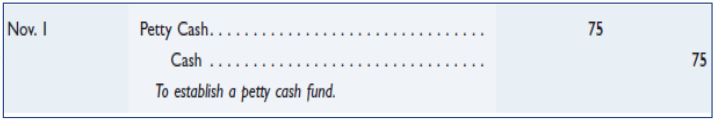
\includegraphics[width=1\columnwidth]{images/c5/establish_petty_cash.png}
		\end{figure}
		\item As petty cash is needed, the petty cashier supplies the cash for 
		the purchases. The petty cash is only used for business expenses
		\item Receipts supporting the petty cash disbursements are given to the 
		petty cashier. Petty cash receipts with either no signature or a forged 
		signature usually indicate misuse of petty cash.
		\begin{figure}[ht]
			\centering
			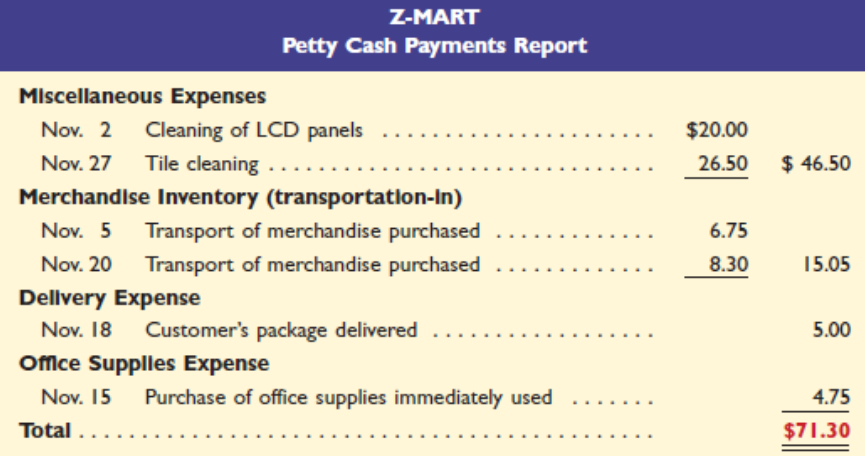
\includegraphics[width=1\columnwidth]{images/c5/payment_cash_payments.png}
			\caption{Petty Cash Payments}
		\end{figure}
		\item When the petty cash fund is low, the petty cashier takes the 
		receipts to the company cashier and requests a check in that amount to 
		replenish the petty cash fund.
		\begin{figure}[ht]
			\centering
			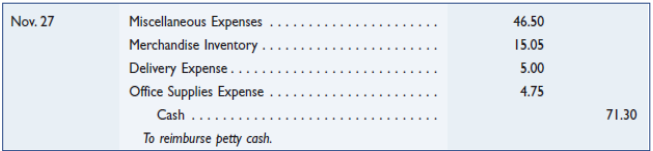
\includegraphics[width=1\columnwidth]{images/c5/reimburse_petty_cash.png}
			\caption{Reimburse Petty Cash}
		\end{figure}
	\end{enumerate}
	
	\subsection{Basic Bank Services}
	
	Banks offer certain protections for your cash. For example,
	\begin{itemize}[noitemsep]
		\item Use of a \textbf{bank account} is a more secure place for your 
		cash than a safe at the office.
		\item \textbf{Signature cards} are used so the bank knows whose 
		signature is approved for use on checks.
		\item \textbf{Deposit slips} provide support for deposits to your 
		account.
		\item \textbf{Checks} provide authorization for disbursements from your 
		account.
		\item \textbf{Electronic funds transfers} limit the number of people 
		who have their hands on the cash and so it reduces theft and fraud.
		\item \textbf{Bank statements} are provided so customers can reconcile 
		their accounts in a timely manner and can detect any unusual or 
		unauthorized activity. 
	\end{itemize}

	\subsection{Controls from Bank Procedures}
	
	Banks provide important services to individuals and businesses. They accept 
	deposits, process payments to others, and provide statements that account 
	for these and other transactions. Their services help businesses to control 
	cash in several ways:
	\begin{itemize}[noitemsep]
		\item \textbf{Restricting access.} Because banks provide a secure place 
		to deposit cash, businesses need to keep only a limited amount of cash 
		on hand, which reduces the risk that it will be stolen or misplaced.
		\item \textbf{Documenting procedures.} By processing payments made by 
		check or EFT, banks facilitate and document business transactions.
		\item \textbf{Independently verifying.} Company accountants can use the 
		statement of account prepared by the bank to double-check the accuracy 
		of the cash records. By comparing these two sets of records and 
		investigating any differences, they can verify that the company’s 
		records are accurate or identify necessary adjustments.
	\end{itemize}
	
	The process of comparing two sets of records is called 
	\textbf{reconciling}. Thus, the internal accounting report that compares 
	the company’s cash records with the bank’s is a bank reconciliation. A bank 
	reconciliation is a key internal control because it provides independent 
	verification of all cash transactions that the bank has processed for the 
	company. This procedure is done monthly, ideally by a company employee 
	whose duties are segregated from recording and handling cash. 
	
	\subsubsection{Bank Statement}
	
	\begin{figure}[ht]
		\centering
		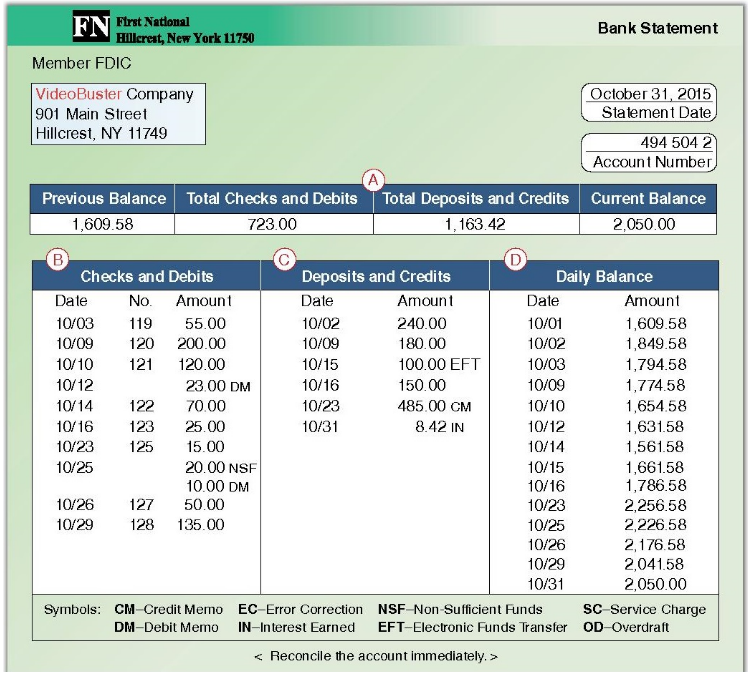
\includegraphics[width=1\columnwidth]{images/c5/bank_statement.png}
		\caption{Bank Statement}
	\end{figure}
	
	Usually, once a month, the bank sends each depositor a bank statement 
	showing the activity in the account. Different banks use different formats 
	for their bank statements, but all of 
	them include the following items of information:
	\begin{itemize}[noitemsep]
		\item Beginning-of-period balance of the depositor’s account.
		\item Checks and other debits decreasing the account during the period. 
		Other debits might include bank service charges or fees, checks 
		deposited that are uncollectible, corrections of previous errors, 
		withdrawals from ATM machines, and periodic payments arranged in 
		advance by the depositor. 
		\item Deposits and other credits increasing the account during the 
		period.
		\item End-of-period balance of the depositor’s account.
	\end{itemize}
	
	\subsubsection{Bank Reconciliation}
	
	A \textbf{bank reconciliation} involves comparing the company’s records to 
	the bank’s statement of account to determine whether they agree. The 
	company’s records can differ from the bank’s records for two basic reasons: 
	
	\begin{itemize}[noitemsep]
		\item The company has recorded some items that the bank doesn’t know 
		about at the time it prepares the statement of account, or
		\item The bank has recorded some items that the company doesn’t know 
		about until the bank statement is examined.
	\end{itemize}
	
	\begin{figure}[ht]
		\centering
		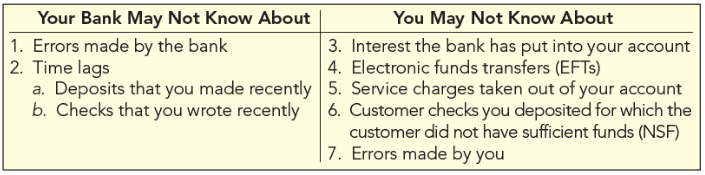
\includegraphics[width=1\columnwidth]{images/c5/bank_reconciliation.png}
		\caption{Bank Reconciliation}
	\end{figure}

	When a company deposits all cash receipts and makes all cash payments 
	(except petty cash) by check, it can use the bank statement for proving the 
	accuracy of its cash records. This is done using a bank reconciliation, 
	which is a report explaining any differences between the checking account 
	balance according to the depositor’s records and the balance reported on 
	the bank statement.
	
	The balance of a checking account reported on the bank statement rarely 
	equals the balance in the depositor’s accounting records. This is usually 
	due to information that one party has that the other does not. We must 
	therefore prove the accuracy of both the depositor’s records and those of 
	the bank. This means we must reconcile the two balances and explain or 
	account for any differences in them. Among the factors causing the bank 
	statement balance to differ from the depositor’s book balance are these:
	\begin{itemize}[noitemsep]
		\item Deposits in transit 
		\item Outstanding checks 
		\item Additions for collections and for interest
		\item Deductions for uncollectible items for services
		\item Errors
	\end{itemize}
	
	\begin{figure}[ht]
		\centering
		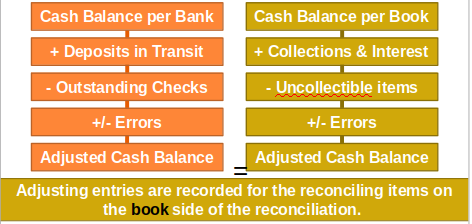
\includegraphics[width=0.7\columnwidth]{images/c5/bank_reconciliation_guidelines.png}
	\end{figure}
	
	When we prepare a bank reconciliation, there are two sections. In one 
	section, we reconcile the bank statement balance to an adjusted bank 
	balance. In the other section, we reconcile the book balance to an adjusted 
	book balance. The adjusted balances in both sections should be equal. After 
	preparing the bank reconciliation, adjusting entries are recorded for the 
	reconciling items on the book side of the reconciliation. 
	
	We follow nine steps in preparing the bank reconciliation:
	\begin{enumerate}[noitemsep]
		\item Identify the bank statement balance of the cash account (balance 
		per bank).
		\item Identify and list any unrecorded deposits and any bank errors 
		understating the bank balance. Add them to the bank balance.
		\item Identify and list any outstanding checks and any bank errors 
		overstating the bank balance. Deduct them from the bank balance.
		\item Compute the adjusted bank balance, also called the corrected or 
		\textbf{reconciled balance}.
		\item Identify the company’s book balance of the cash account (balance 
		per book).
		\item Identify and list any unrecorded credit memoranda from the bank, 
		any interest earned, and errors understating the book balance. Add them 
		to the book balance.
		\item Identify and list any unrecorded debit memoranda from the bank, 
		any service charges, and errors overstating the book balance. Deduct 
		them from the book balance.
		\item Compute the adjusted book balance, also called corrected or 
		\textbf{reconciled balance}.
		\item Verify that the two adjusted balances from steps 4 and 8 are 
		equal. If so, they are reconciled. If not, check for accuracy and 
		missing data to achieve reconciliation.
	\end{enumerate}
	
	Only the items reconciling the book balance requires adjustment. 
	
	
	\begin{figure}[ht]
		\centering
		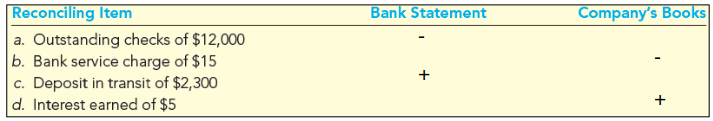
\includegraphics[width=1\columnwidth]{images/c5/reconciliation_example.png}
	\end{figure}

	\subsubsection{Speeding up Cash Collection}
	
	An important part of cash management is monitoring the receipt of cash 
		from receivables. If 
	customers and others who owe money to a company are delayed in payment, 
	then that company can find 
	it difficult to pay its obligations when they are due. A company’s 
	customers are crucial partners 
	in its cash management. Many companies attract customers by selling to them 
	on credit. This means 
	that cash receipts from customers are delayed until accounts receivable are 
	collected. 
	
	One measure 
	of how quickly a company can convert its accounts receivable into cash is 
	the days’ sales 
	uncollected, also called days’ sales in receivables. This measure is 
	computed by dividing the 
	current balance of receivables by net credit sales over the year just 
	completed and then 
	multiplying by 365 (number of days in a year). Since net credit sales 
	usually are not reported to 
	external users, the net sales (or revenues) figure is commonly used in the 
	computation.
		
	One way to speed up collections is to sell outstanding accounts 
	receivable to another company (called a \textbf{factor}). The way a 
	factoring 
	arrangement is that your company receives cash for the receivables it sells 
	to the factor (minus a \textbf{factoring fee}) and the factor then has the 
	right to collect the outstanding amounts owed by your customers. 
	\textbf{Factoring} is a fast and 
	easy way for your company to get cash for its receivables but with costs.
	
	Another way to avoid lengthy collection periods is to allow customers to 
	pay for goods using PayPal or credit cards. Some banks accept credit card 
	receipts as overnight deposits into the company’s bank account as if 
	they’re cash. This not only speeds up the seller’s cash collection, but 
	also reduces losses from customers writing bad checks. Remember, just like 
	the factor, PayPal and the credit card companies charge a fee for their 
	services.
	
	
\end{document}